% Options for packages loaded elsewhere
\PassOptionsToPackage{unicode}{hyperref}
\PassOptionsToPackage{hyphens}{url}
%
\documentclass[
]{article}
\usepackage{lmodern}
\usepackage{amssymb,amsmath}
\usepackage{ifxetex,ifluatex}
\ifnum 0\ifxetex 1\fi\ifluatex 1\fi=0 % if pdftex
  \usepackage[T1]{fontenc}
  \usepackage[utf8]{inputenc}
  \usepackage{textcomp} % provide euro and other symbols
\else % if luatex or xetex
  \usepackage{unicode-math}
  \defaultfontfeatures{Scale=MatchLowercase}
  \defaultfontfeatures[\rmfamily]{Ligatures=TeX,Scale=1}
\fi
% Use upquote if available, for straight quotes in verbatim environments
\IfFileExists{upquote.sty}{\usepackage{upquote}}{}
\IfFileExists{microtype.sty}{% use microtype if available
  \usepackage[]{microtype}
  \UseMicrotypeSet[protrusion]{basicmath} % disable protrusion for tt fonts
}{}
\makeatletter
\@ifundefined{KOMAClassName}{% if non-KOMA class
  \IfFileExists{parskip.sty}{%
    \usepackage{parskip}
  }{% else
    \setlength{\parindent}{0pt}
    \setlength{\parskip}{6pt plus 2pt minus 1pt}}
}{% if KOMA class
  \KOMAoptions{parskip=half}}
\makeatother
\usepackage{xcolor}
\IfFileExists{xurl.sty}{\usepackage{xurl}}{} % add URL line breaks if available
\IfFileExists{bookmark.sty}{\usepackage{bookmark}}{\usepackage{hyperref}}
\hypersetup{
  hidelinks,
  pdfcreator={LaTeX via pandoc}}
\urlstyle{same} % disable monospaced font for URLs
\usepackage[left=1cm,right=1cm,top=1.8cm,bottom=1.25cm]{geometry}
\usepackage{graphicx,grffile}
\makeatletter
\def\maxwidth{\ifdim\Gin@nat@width>\linewidth\linewidth\else\Gin@nat@width\fi}
\def\maxheight{\ifdim\Gin@nat@height>\textheight\textheight\else\Gin@nat@height\fi}
\makeatother
% Scale images if necessary, so that they will not overflow the page
% margins by default, and it is still possible to overwrite the defaults
% using explicit options in \includegraphics[width, height, ...]{}
\setkeys{Gin}{width=\maxwidth,height=\maxheight,keepaspectratio}
% Set default figure placement to htbp
\makeatletter
\def\fps@figure{htbp}
\makeatother
\setlength{\emergencystretch}{3em} % prevent overfull lines
\providecommand{\tightlist}{%
  \setlength{\itemsep}{0pt}\setlength{\parskip}{0pt}}
\setcounter{secnumdepth}{-\maxdimen} % remove section numbering
\usepackage{fancyhdr} \pagestyle{fancy} \usepackage{graphicx} \usepackage{eurosym} \usepackage{xcolor} \usepackage{booktabs,xcolor} \definecolor{myblue}{HTML}{5F7ED9} \definecolor{wblight}{HTML}{f8f4fc} \definecolor{wbmid}{HTML}{f0ecfc} \definecolor{wbpurple}{HTML}{c8c4ec} \definecolor{wbfemale}{HTML}{303c84} \definecolor{wbmale}{HTML}{707cbc} \lfoot{\mbox{\kern\dimexpr-1cm
\includegraphics[width=\paperwidth]{footer.png}}} \fancypagestyle{plain}{\pagestyle{fancy}} \pagenumbering{gobble} \usepackage[defaultfam,tabular,lining]{montserrat} \usepackage[fontsize=8pt]{scrextend} \usepackage{float} \restylefloat{table} \usepackage{multicol} \usepackage{paralist} \usepackage{hyperref} \newcommand{\hideFromPandoc}[1]{#1} \hideFromPandoc{ \let\Begin\begin \let\End\end } \usepackage{caption} \usepackage[framemethod=tikz]{mdframed} \newmdenv[innerlinewidth=0.5pt, roundcorner=24pt,linecolor=white,backgroundcolor=wbpurple,innerleftmargin=2pt,innerrightmargin=2pt,innertopmargin=2pt,innerbottommargin=0pt,nobreak=True,leftmargin = 3.5pt,rightmargin = 3.5pt]{mybox} \newcommand*\circled[1]{\tikz[baseline=(char.base)]{ \node[shape=circle,text width=30pt,align=center,draw=wbpurple,minimum size=30pt,outer sep=0pt,fill=wblight] (char) {#1};}} \newcommand*\squared[1]{\tikz[baseline=(char.base)]{ \node[shape=rectangle,text width=3.15cm,align=center,draw=wbpurple,minimum size=1.5cm,outer sep=0pt,inner sep=4pt,fill=wblight] (char) {#1};}} \captionsetup{skip=0pt} \setlength{\headsep}{.65cm}
\usepackage{booktabs}
\usepackage{longtable}
\usepackage{array}
\usepackage{multirow}
\usepackage{wrapfig}
\usepackage{float}
\usepackage{colortbl}
\usepackage{pdflscape}
\usepackage{tabu}
\usepackage{threeparttable}
\usepackage{threeparttablex}
\usepackage[normalem]{ulem}
\usepackage{makecell}
\usepackage{xcolor}

\author{}
\date{\vspace{-2.5em}}

\begin{document}

\lhead{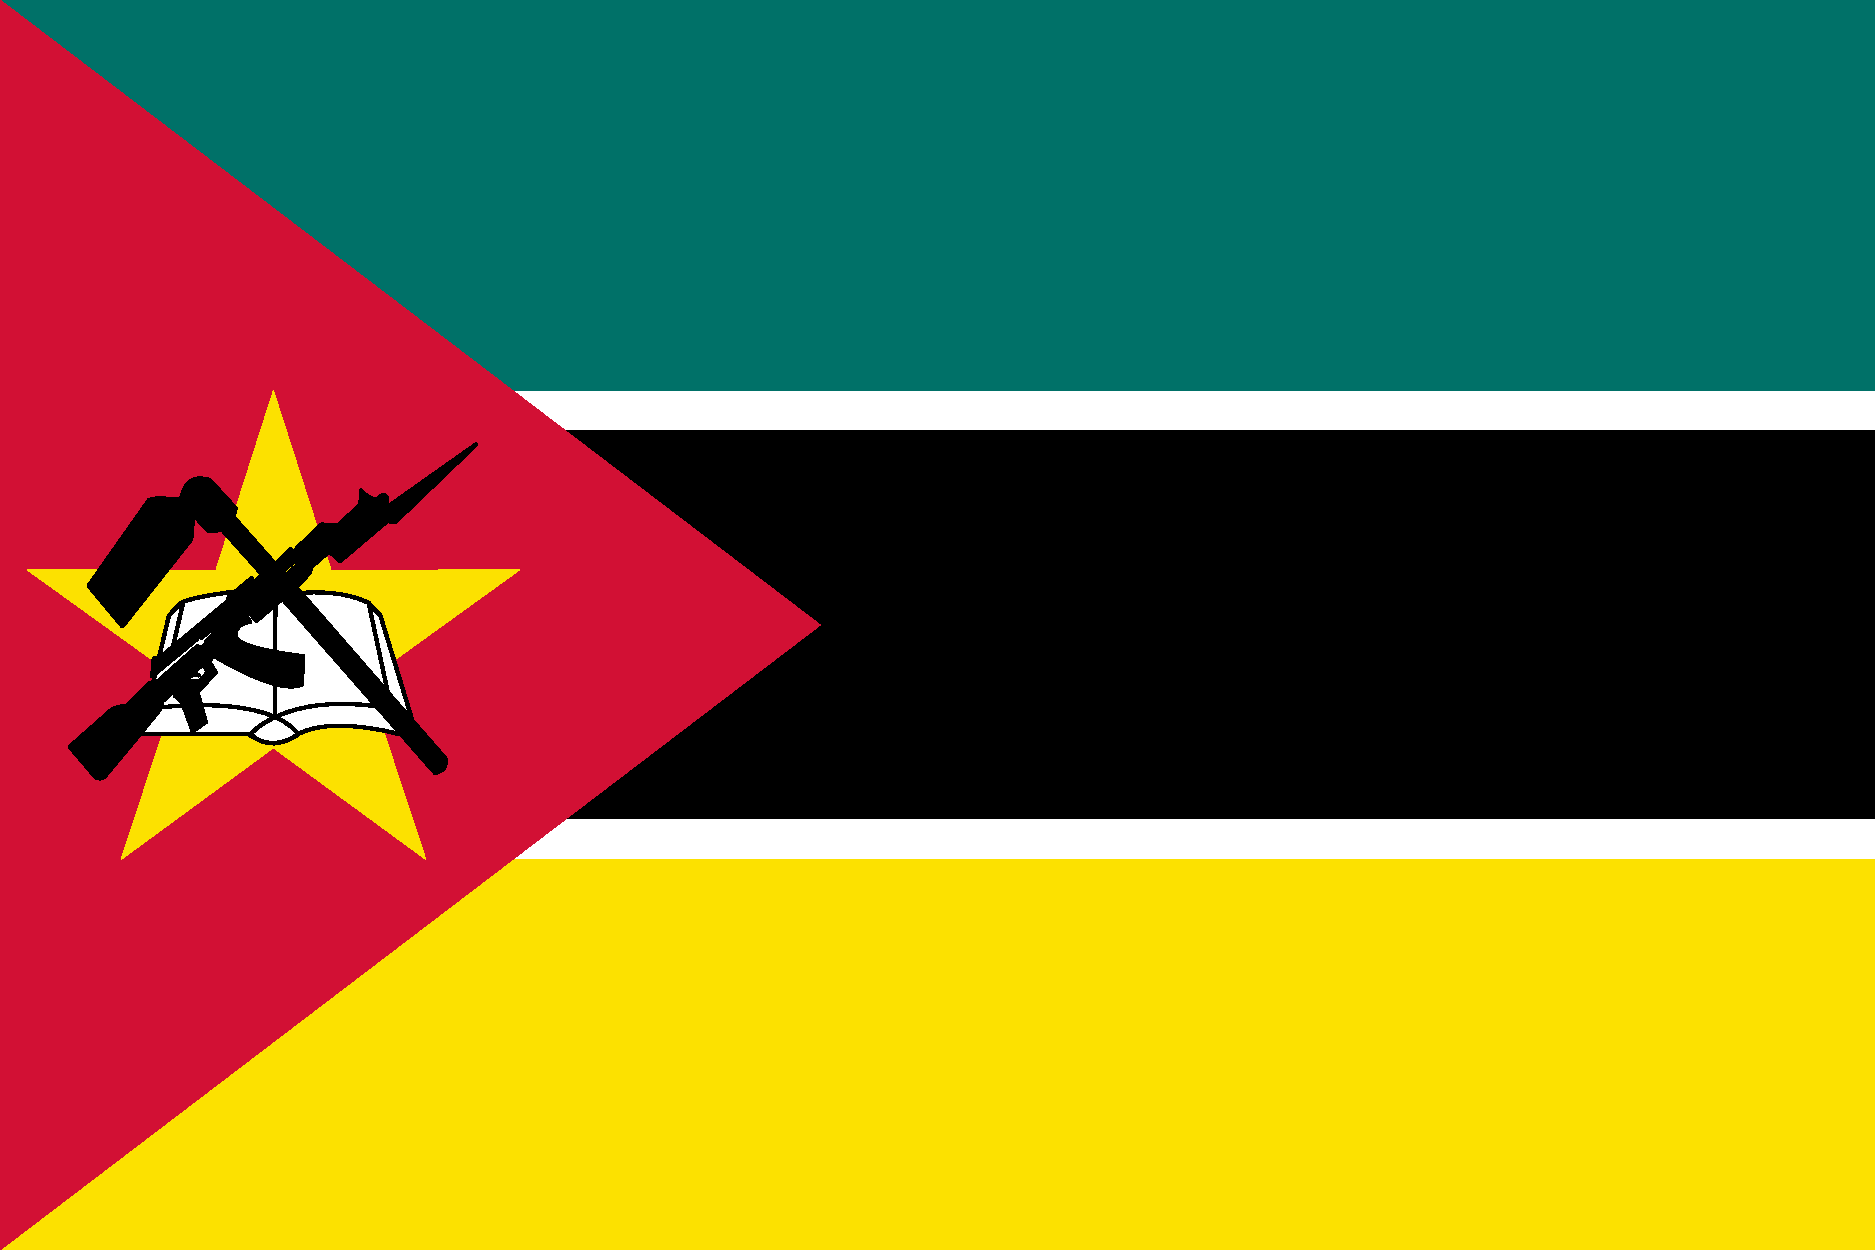
\includegraphics[width=1cm]{pdf/mz.pdf}\fontsize{22}{1}\selectfont\textbf{\  MOZAMBIQUE \textcolor{myblue}{GENDER LANDSCAPE}}}

\begin{wraptable}{r}{0pt}\begingroup\fontsize{8}{10}\selectfont

\begin{tabular}[t]{lcl}

\textbf{Compared to:} & \textbf{Base Year} & \textbf{Region}\\
\midrule
>10\% Higher Value & 
\includegraphics[width=0.1in, height=0.1in]{upicon.png} & \cellcolor[HTML]{21908C}{}\\
Equal/No Change & 
\includegraphics[width=0.1in, height=0.1in]{righticon.png} & \cellcolor[HTML]{34608D}{}\\
>10\% Lower Value & 
\includegraphics[width=0.1in, height=0.1in]{downicon.png} & \cellcolor[HTML]{482576}{}\\
No Data & 
\includegraphics[width=0.1in, height=0.1in]{naicon.png} & \cellcolor{gray}{}\\

\end{tabular}
\endgroup{}\end{wraptable}
\begin{minipage}[t][1.7cm][t]{12cm}
\fontsize{9}{8}\selectfont\raggedright
This briefing showcases the gender landscape in Mozambique on key indicators helpful for monitoring gender equality and designing effective policy interventions. Gender equality fosters productivity gains and minimizes losses in wealth, reduces poverty, boosts shared prosperity, and supports green, resilient, and inclusive development. 


\includegraphics[width=10pt]{pointer.png} Click the links below to explore the \underline{\href{https://genderdata.worldbank.org/}{World Bank Gender Data Portal}}.
\end{minipage}
\vspace{8pt}

\begingroup\fontsize{7.5}{9.5}\selectfont

\begin{ThreePartTable}
\begin{TableNotes}[para]
\item \textit{Note: } 
\item \textcolor{darkgray}{Data retrieved from \underline{\href{https://genderdata.worldbank.org/}{World Bank Gender Data Portal}}. The Sub-Saharan Africa (SSA)  region includes 48 countries (all income levels), as classified by The World Bank Group. Mozambique is a Low income (LIC) country, which includes 27 countries with a Gross National Income (GNI) per capita from \$0 to \$1,045 (calculated using the World Bank Atlas method). Data definitions can be found on the \underline{\href{https://genderdata.worldbank.org/}{Gender Data Portal}}.} 

\textcolor{darkgray}{Country Baseline provides a reference value between 1990 and 2010. Latest Value shows the latest available comparison from 2011 onwards. Baseline comparisons are represented by an arrow icon that points to increases or decreases greater than 10 percent relative to the base year. Comparison to the regional average shows how Mozambique performs relative to its peers in the region, income group, and the world. Darker and lighter shades represent values 10 percent or below or above its peers in the region, respectively.}
\end{TableNotes}
\begin{longtable}[t]{>{\raggedright\arraybackslash}p{9cm}>{\raggedright\arraybackslash}p{1.1cm}>{}c>{}c>{}c>{}c>{}c>{}c>{}c>{}c}
\toprule
\multicolumn{2}{c}{\textbf{ }} & \multicolumn{5}{c}{\textbf{Country Performance}} & \multicolumn{3}{c}{\textbf{Peer Comparison}} \\
\cmidrule(l{3pt}r{3pt}){3-7} \cmidrule(l{3pt}r{3pt}){8-10}
\multicolumn{2}{c}{\textbf{ }} & \multicolumn{2}{c}{\textbf{Baseline}} & \multicolumn{1}{c}{\textbf{ }} & \multicolumn{2}{c}{\textbf{Latest}} & \multicolumn{3}{c}{\textbf{Latest}} \\
\cmidrule(l{3pt}r{3pt}){3-4} \cmidrule(l{3pt}r{3pt}){6-7} \cmidrule(l{3pt}r{3pt}){8-10}
\textbf{\textbf{}} & \textbf{\textbf{}} & \textbf{\textbf{Value}} & \textbf{\textbf{Year}} & \textbf{\textbf{}} & \textbf{\textbf{Value}} & \textbf{\textbf{Year}} & \textbf{\textbf{SSA}} & \textbf{\textbf{LIC}} & \textbf{\textbf{World}}\\
\midrule
\endfirsthead
\multicolumn{10}{@{}l}{\textit{(continued)}}\\
\toprule
\textbf{\textbf{}} & \textbf{\textbf{}} & \textbf{\textbf{Value}} & \textbf{\textbf{Year}} & \textbf{\textbf{}} & \textbf{\textbf{Value}} & \textbf{\textbf{Year}} & \textbf{\textbf{SSA}} & \textbf{\textbf{LIC}} & \textbf{\textbf{World}}\\
\midrule
\endhead

\endfoot
\bottomrule
\insertTableNotes
\endlastfoot
\addlinespace[0.3em]
\multicolumn{10}{l}{\cellcolor{lightgray}{\textbf{HUMAN ENDOWMENTS}}}\\
 & Female & \textcolor{gray}{NA} & \textcolor{gray}{NA} & 
\includegraphics[width=0.1in, height=0.1in]{naicon.png} & \cellcolor{gray}{\textcolor{white}{\textbf{NA}}} & \textcolor{gray}{NA} & \textcolor{gray}{NA} & \textcolor{gray}{NA} & \textcolor{gray}{NA}\\
\nopagebreak
\multirow{-2}{9cm}{\raggedright\arraybackslash \href{https://genderdata.worldbank.org/indicators/hd-hci-lays/}{Learning-Adjusted Years of School}} & Male & \textcolor{gray}{NA} & \textcolor{gray}{NA} & 
\includegraphics[width=0.1in, height=0.1in]{naicon.png} & \cellcolor{gray}{\textcolor{white}{\textbf{NA}}} & \textcolor{gray}{NA} & \textcolor{gray}{NA} & \textcolor{gray}{NA} & \textcolor{gray}{NA}\\
\cmidrule{1-10}\pagebreak[0]
 & Female & \textcolor[HTML]{000004}{36.5} & \textcolor[HTML]{000004}{2009} & 
\includegraphics[width=0.1in, height=0.1in]{upicon.png} & \cellcolor[HTML]{482576}{\textcolor{white}{\textbf{50.3}}} & \textcolor[HTML]{000004}{2017} & \textcolor[HTML]{000004}{59.4} & \textcolor[HTML]{000004}{54.1} & \textcolor[HTML]{000004}{83.3}\\
\nopagebreak
\multirow{-2}{9cm}{\raggedright\arraybackslash \href{https://genderdata.worldbank.org/indicators/se-adt/}{Literacy rate (\% age 15+)}} & Male & \textcolor[HTML]{000004}{67.4} & \textcolor[HTML]{000004}{2009} & 
\includegraphics[width=0.1in, height=0.1in]{righticon.png} & \cellcolor[HTML]{355F8D}{\textcolor{white}{\textbf{72.6}}} & \textcolor[HTML]{000004}{2017} & \textcolor[HTML]{000004}{72.5} & \textcolor[HTML]{000004}{68.9} & \textcolor[HTML]{000004}{90.1}\\
\cmidrule{1-10}\pagebreak[0]
 & Female & \textcolor[HTML]{000004}{18.9} & \textcolor[HTML]{000004}{2010} & 
\includegraphics[width=0.1in, height=0.1in]{upicon.png} & \cellcolor[HTML]{482576}{\textcolor{white}{\textbf{24.3}}} & \textcolor[HTML]{000004}{2019} & \textcolor[HTML]{000004}{41.3} & \textcolor[HTML]{000004}{35.3} & \textcolor[HTML]{000004}{77.3}\\
\nopagebreak
\multirow{-2}{9cm}{\raggedright\arraybackslash \href{https://genderdata.worldbank.org/indicators/se-sec-cmpt-lo-zs}{Lower secondary completion rate (\% of relevant age group)}} & Male & \textcolor[HTML]{000004}{23.4} & \textcolor[HTML]{000004}{2010} & 
\includegraphics[width=0.1in, height=0.1in]{righticon.png} & \cellcolor[HTML]{482576}{\textcolor{white}{\textbf{24.1}}} & \textcolor[HTML]{000004}{2019} & \textcolor[HTML]{000004}{46.0} & \textcolor[HTML]{000004}{43.1} & \textcolor[HTML]{000004}{76.7}\\
\cmidrule{1-10}\pagebreak[0]
\href{https://genderdata.worldbank.org/indicators/sp-dyn-tfrt-in/}{Fertility rate, total (births per woman)} &  & \textcolor[HTML]{000004}{5.39} & \textcolor[HTML]{000004}{2010} & 
\includegraphics[width=0.1in, height=0.1in]{downicon.png} & \cellcolor[HTML]{355F8D}{\textcolor{white}{\textbf{4.71}}} & \textcolor[HTML]{000004}{2020} & \textcolor[HTML]{000004}{4.56} & \textcolor[HTML]{000004}{4.49} & \textcolor[HTML]{000004}{2.39}\\
\cmidrule{1-10}\pagebreak[0]
\href{https://genderdata.worldbank.org/indicators/sp-ado-tfrt/}{Adolescent fertility rate (births per 1,000 women ages 15-19)} &  & \textcolor[HTML]{000004}{164} & \textcolor[HTML]{000004}{2010} & 
\includegraphics[width=0.1in, height=0.1in]{downicon.png} & \cellcolor[HTML]{21908C}{\textcolor{white}{\textbf{142}}} & \textcolor[HTML]{000004}{2020} & \textcolor[HTML]{000004}{98.0} & \textcolor[HTML]{000004}{91.8} & \textcolor[HTML]{000004}{41.0}\\
\cmidrule{1-10}\pagebreak[0]
\href{https://genderdata.worldbank.org/indicators/sp-uwt-tfrt}{Unmet need for contraception (\% of married women ages 15-49)} &  & \textcolor[HTML]{000004}{18.9} & \textcolor[HTML]{000004}{2004} & 
\includegraphics[width=0.1in, height=0.1in]{upicon.png} & \cellcolor[HTML]{355F8D}{\textcolor{white}{\textbf{23.1}}} & \textcolor[HTML]{000004}{2015} & \textcolor[HTML]{000004}{22.6} & \textcolor[HTML]{000004}{23.5} & \textcolor{gray}{NA}\\
\cmidrule{1-10}\pagebreak[0]
\href{https://genderdata.worldbank.org/indicators/sh-sta-anv-4-zs}{Pregnant women receiving prenatal care of at least four visits (\% of pregnant women)} &  & \textcolor[HTML]{000004}{52.9} & \textcolor[HTML]{000004}{2003} & 
\includegraphics[width=0.1in, height=0.1in]{righticon.png} & \cellcolor{gray}{\textcolor{white}{\textbf{48.6}}} & \textcolor[HTML]{000004}{2011} & \textcolor{gray}{NA} & \textcolor{gray}{NA} & \textcolor{gray}{NA}\\
\cmidrule{1-10}\pagebreak[0]
\href{https://genderdata.worldbank.org/indicators/sh-sta-mmrt/}{Maternal mortality ratio (modeled estimate per 100,000 live births)} &  & \textcolor[HTML]{000004}{412} & \textcolor[HTML]{000004}{2010} & 
\includegraphics[width=0.1in, height=0.1in]{downicon.png} & \cellcolor[HTML]{482576}{\textcolor{white}{\textbf{289}}} & \textcolor[HTML]{000004}{2017} & \textcolor[HTML]{000004}{534} & \textcolor[HTML]{000004}{460} & \textcolor[HTML]{000004}{211}\\
\cmidrule{1-10}\pagebreak[0]
 & Female & \textcolor[HTML]{000004}{24.4} & \textcolor[HTML]{000004}{2010} & 
\includegraphics[width=0.1in, height=0.1in]{righticon.png} & \cellcolor[HTML]{21908C}{\textcolor{white}{\textbf{23.9}}} & \textcolor[HTML]{000004}{2019} & \textcolor[HTML]{000004}{20.1} & \textcolor[HTML]{000004}{21.7} & \textcolor[HTML]{000004}{14.8}\\
\nopagebreak
\multirow{-2}{9cm}{\raggedright\arraybackslash \href{https://genderdata.worldbank.org/indicators/sh-dyn-ncom-zs}{Mortality from chronic vascular disease, cancer, diabetes or cardiorespiratory disease between 30 and 70 (\%)}} & Male & \textcolor[HTML]{000004}{41.8} & \textcolor[HTML]{000004}{2010} & 
\includegraphics[width=0.1in, height=0.1in]{righticon.png} & \cellcolor[HTML]{21908C}{\textcolor{white}{\textbf{38.8}}} & \textcolor[HTML]{000004}{2019} & \textcolor[HTML]{000004}{22.7} & \textcolor[HTML]{000004}{25.4} & \textcolor[HTML]{000004}{21.7}\\
\cmidrule{1-10}\pagebreak[0]
\addlinespace[0.3em]
\multicolumn{10}{l}{\cellcolor{lightgray}{\textbf{ECONOMIC OPPORTUNITY}}}\\
 & Female & \textcolor[HTML]{000004}{82.7} & \textcolor[HTML]{000004}{2010} & 
\includegraphics[width=0.1in, height=0.1in]{righticon.png} & \cellcolor[HTML]{21908C}{\textcolor{white}{\textbf{77.7}}} & \textcolor[HTML]{000004}{2021} & \textcolor[HTML]{000004}{60.2} & \textcolor[HTML]{000004}{56.8} & \textcolor[HTML]{000004}{46.3}\\
\nopagebreak
\multirow{-2}{9cm}{\raggedright\arraybackslash \href{https://genderdata.worldbank.org/indicators/sl-tlf-acti-zs/}{Labor force participation rate (\% age 15+, modeled ILO estimate)}} & Male & \textcolor[HTML]{000004}{81.7} & \textcolor[HTML]{000004}{2010} & 
\includegraphics[width=0.1in, height=0.1in]{righticon.png} & \cellcolor[HTML]{21908C}{\textcolor{white}{\textbf{78.9}}} & \textcolor[HTML]{000004}{2021} & \textcolor[HTML]{000004}{71.7} & \textcolor[HTML]{000004}{74.9} & \textcolor[HTML]{000004}{71.7}\\
\cmidrule{1-10}\pagebreak[0]
 & Female & \textcolor[HTML]{000004}{4.37} & \textcolor[HTML]{000004}{2010} & 
\includegraphics[width=0.1in, height=0.1in]{upicon.png} & \cellcolor[HTML]{482576}{\textcolor{white}{\textbf{6.84}}} & \textcolor[HTML]{000004}{2019} & \textcolor[HTML]{000004}{18.8} & \textcolor[HTML]{000004}{13.2} & \textcolor[HTML]{000004}{54.6}\\
\nopagebreak
\multirow{-2}{9cm}{\raggedright\arraybackslash \href{https://genderdata.worldbank.org/indicators/sl-emp-work-zs}{Wage and salaried workers (\% of employment, modeled ILO estimate)}} & Male & \textcolor[HTML]{000004}{19.1} & \textcolor[HTML]{000004}{2010} & 
\includegraphics[width=0.1in, height=0.1in]{upicon.png} & \cellcolor[HTML]{482576}{\textcolor{white}{\textbf{25.4}}} & \textcolor[HTML]{000004}{2019} & \textcolor[HTML]{000004}{30.4} & \textcolor[HTML]{000004}{24.9} & \textcolor[HTML]{000004}{53.0}\\
\cmidrule{1-10}\pagebreak[0]
 & Female & \textcolor[HTML]{000004}{86.4} & \textcolor[HTML]{000004}{2010} & 
\includegraphics[width=0.1in, height=0.1in]{righticon.png} & \cellcolor[HTML]{21908C}{\textcolor{white}{\textbf{79.8}}} & \textcolor[HTML]{000004}{2019} & \textcolor[HTML]{000004}{52.6} & \textcolor[HTML]{000004}{63.4} & \textcolor[HTML]{000004}{25.3}\\
\nopagebreak
\multirow{-2}{9cm}{\raggedright\arraybackslash \href{https://genderdata.worldbank.org/indicators/sl-empl-zs}{Employment in agriculture (\% of employment, modeled ILO estimate)}} & Male & \textcolor[HTML]{000004}{64.9} & \textcolor[HTML]{000004}{2010} & 
\includegraphics[width=0.1in, height=0.1in]{righticon.png} & \cellcolor[HTML]{21908C}{\textcolor{white}{\textbf{59.8}}} & \textcolor[HTML]{000004}{2019} & \textcolor[HTML]{000004}{53.2} & \textcolor[HTML]{000004}{56.9} & \textcolor[HTML]{000004}{27.6}\\
\cmidrule{1-10}\pagebreak[0]
 & Female & \textcolor{gray}{NA} & \textcolor{gray}{NA} & 
\includegraphics[width=0.1in, height=0.1in]{naicon.png} & \cellcolor{gray}{\textcolor{white}{\textbf{NA}}} & \textcolor{gray}{NA} & \textcolor{gray}{NA} & \textcolor{gray}{NA} & \textcolor{gray}{NA}\\
\nopagebreak
\multirow{-2}{9cm}{\raggedright\arraybackslash \href{https://genderdata.worldbank.org/indicators/sl-uem-neet-zs/}{Share of youth not in education, employment or training (\% of youth population)}} & Male & \textcolor{gray}{NA} & \textcolor{gray}{NA} & 
\includegraphics[width=0.1in, height=0.1in]{naicon.png} & \cellcolor{gray}{\textcolor{white}{\textbf{NA}}} & \textcolor{gray}{NA} & \textcolor{gray}{NA} & \textcolor{gray}{NA} & \textcolor{gray}{NA}\\
\cmidrule{1-10}\pagebreak[0]
\href{https://genderdata.worldbank.org/indicators/sp-pop-dpnd}{Age dependency ratio (\% of working-age population)} &  & \textcolor[HTML]{000004}{95.1} & \textcolor[HTML]{000004}{2010} & 
\includegraphics[width=0.1in, height=0.1in]{righticon.png} & \cellcolor[HTML]{355F8D}{\textcolor{white}{\textbf{88.4}}} & \textcolor[HTML]{000004}{2020} & \textcolor[HTML]{000004}{82.6} & \textcolor[HTML]{000004}{82.8} & \textcolor[HTML]{000004}{54.6}\\
\cmidrule{1-10}\pagebreak[0]
\href{https://genderdata.worldbank.org/indicators/sg-own-ld}{Women who own land both alone and jointly (\% of women age 15-49)} &  & \textcolor{gray}{NA} & \textcolor{gray}{NA} & 
\includegraphics[width=0.1in, height=0.1in]{naicon.png} & \cellcolor{gray}{\textcolor{white}{\textbf{2.40}}} & \textcolor[HTML]{000004}{2015} & \textcolor{gray}{NA} & \textcolor{gray}{NA} & \textcolor{gray}{NA}\\
\cmidrule{1-10}\pagebreak[0]
 & Female & \textcolor{gray}{NA} & \textcolor{gray}{NA} & 
\includegraphics[width=0.1in, height=0.1in]{naicon.png} & \cellcolor{gray}{\textcolor{white}{\textbf{26.3}}} & \textcolor[HTML]{000004}{2017} & \textcolor{gray}{NA} & \textcolor[HTML]{000004}{20.5} & \textcolor[HTML]{000004}{63.7}\\
\nopagebreak
\multirow{-2}{9cm}{\raggedright\arraybackslash \href{https://genderdata.worldbank.org/indicators/fin1-t-a/}{Financial institution account (\% age 15+)}} & Male & \textcolor{gray}{NA} & \textcolor{gray}{NA} & 
\includegraphics[width=0.1in, height=0.1in]{naicon.png} & \cellcolor{gray}{\textcolor{white}{\textbf{40.2}}} & \textcolor[HTML]{000004}{2017} & \textcolor{gray}{NA} & \textcolor[HTML]{000004}{28.7} & \textcolor[HTML]{000004}{70.6}\\
\cmidrule{1-10}\pagebreak[0]
 & Female & \textcolor{gray}{NA} & \textcolor{gray}{NA} & 
\includegraphics[width=0.1in, height=0.1in]{naicon.png} & \cellcolor{gray}{\textcolor{white}{\textbf{7.12}}} & \textcolor[HTML]{000004}{2017} & \textcolor{gray}{NA} & \textcolor[HTML]{000004}{10.6} & \textcolor[HTML]{000004}{5.26}\\
\nopagebreak
\multirow{-2}{9cm}{\raggedright\arraybackslash \href{https://genderdata.worldbank.org/indicators/fin15-t-a}{Borrowed to start, operate, or expand a farm or business (\% age 15+)}} & Male & \textcolor{gray}{NA} & \textcolor{gray}{NA} & 
\includegraphics[width=0.1in, height=0.1in]{naicon.png} & \cellcolor{gray}{\textcolor{white}{\textbf{10.7}}} & \textcolor[HTML]{000004}{2017} & \textcolor{gray}{NA} & \textcolor[HTML]{000004}{12.8} & \textcolor[HTML]{000004}{7.57}\\
\cmidrule{1-10}\pagebreak[0]
\href{https://genderdata.worldbank.org/indicators/ic-wef-llco-zs/}{Firms with female participation in ownership (\% of firms)} &  & \textcolor[HTML]{000004}{24.4} & \textcolor[HTML]{000004}{2007} & 
\includegraphics[width=0.1in, height=0.1in]{upicon.png} & \cellcolor[HTML]{355F8D}{\textcolor{white}{\textbf{28.3}}} & \textcolor[HTML]{000004}{2018} & \textcolor[HTML]{000004}{28.0} & \textcolor[HTML]{000004}{23.3} & \textcolor[HTML]{000004}{33.1}\\
\cmidrule{1-10}\pagebreak[0]
\addlinespace[0.3em]
\multicolumn{10}{l}{\cellcolor{lightgray}{\textbf{VOICE AND AGENCY}}}\\
\href{https://genderdata.worldbank.org/indicators/ic-frm-femm-zs/}{Firms with female top manager (\% of firms)} &  & \textcolor{gray}{NA} & \textcolor{gray}{NA} & 
\includegraphics[width=0.1in, height=0.1in]{naicon.png} & \cellcolor[HTML]{355F8D}{\textcolor{white}{\textbf{15.6}}} & \textcolor[HTML]{000004}{2018} & \textcolor[HTML]{000004}{16.2} & \textcolor[HTML]{000004}{12.2} & \textcolor[HTML]{000004}{17.8}\\
\cmidrule{1-10}\pagebreak[0]
\href{https://genderdata.worldbank.org/indicators/sg-gen-parl-zs/}{Proportion of seats held by women in national parliaments (\%)} &  & \textcolor[HTML]{000004}{39.2} & \textcolor[HTML]{000004}{2010} & 
\includegraphics[width=0.1in, height=0.1in]{righticon.png} & \cellcolor[HTML]{21908C}{\textcolor{white}{\textbf{42.4}}} & \textcolor[HTML]{000004}{2021} & \textcolor[HTML]{000004}{25.9} & \textcolor[HTML]{000004}{24.1} & \textcolor[HTML]{000004}{26.1}\\
\cmidrule{1-10}\pagebreak[0]
\href{https://genderdata.worldbank.org/indicators/sp-2024-fe-zs/}{Women who were first married by age 18 (\% of women ages 20-24)} &  & \textcolor[HTML]{000004}{56.2} & \textcolor[HTML]{000004}{2009} & 
\includegraphics[width=0.1in, height=0.1in]{righticon.png} & \cellcolor{gray}{\textcolor{white}{\textbf{52.9}}} & \textcolor[HTML]{000004}{2015} & \textcolor{gray}{NA} & \textcolor{gray}{NA} & \textcolor{gray}{NA}\\
\cmidrule{1-10}\pagebreak[0]
\href{https://genderdata.worldbank.org/indicators/sg-vaw-1549-zs/}{Proportion of women subjected to physical and/or sexual violence in the last 12 months (\% of ever-partnered women ages 15-49)} &  & \textcolor{gray}{NA} & \textcolor{gray}{NA} & 
\includegraphics[width=0.1in, height=0.1in]{naicon.png} & \cellcolor{gray}{\textcolor{white}{\textbf{15.5}}} & \textcolor[HTML]{000004}{2015} & \textcolor{gray}{NA} & \textcolor{gray}{NA} & \textcolor{gray}{NA}\\
\cmidrule{1-10}\pagebreak[0]
\href{https://genderdata.worldbank.org/indicators/sg-vaw-zs}{Women who believe a husband is justified in beating his wife (any of five reasons, \%)} &  & \textcolor[HTML]{000004}{54.1} & \textcolor[HTML]{000004}{2003} & 
\includegraphics[width=0.1in, height=0.1in]{downicon.png} & \cellcolor{gray}{\textcolor{white}{\textbf{13.3}}} & \textcolor[HTML]{000004}{2015} & \textcolor{gray}{NA} & \textcolor{gray}{NA} & \textcolor{gray}{NA}\\*
\end{longtable}
\end{ThreePartTable}
\endgroup{}

\newpage
\clearpage

\raggedright
\vspace{.2cm}
\fcolorbox{white}{white}{\color{black}
\begin{minipage}[c][1.4cm][t]{19.5cm}
\begin{minipage}[c][1.4cm][t]{6.5cm}
\fontsize{14}{1}\selectfont   
Women, Business and
  
\vspace{.2cm}
  
the Law in Mozambique
\normalsize
\end{minipage}
\begin{minipage}[c][1.4cm][t]{12.75cm}
\fontsize{9}{8}\selectfont   
\textbf{\underline{\href{https://wbl.worldbank.org/en/wbl}{Women, Business and the Law (WBL) 2022}}} presents an index covering 190 economies, structured around the life cycle of a working woman. In total, 35 questions are scored across eight indicators. \textbf{Mozambique scores 82.5 out of 100,} while the regional average across Sub-Saharan Africa is 80.4.
\normalsize
\end{minipage}
\end{minipage}}

\centering
\begin{minipage}[c][4.2cm][t]{2.1cm}\begin{mybox}\centering
\vspace{.3cm}

\includegraphics[height=.75cm]{overall.png}

\vspace{.3cm}
\fontsize{7.5}{1}\selectfont   
\textbf{{\href{https://genderdata.worldbank.org/indicators/sg-law-indx}{Overall}}}\normalsize 

\vspace{12pt}
\fontsize{14}{1}\selectfont 
\centering\tikz[baseline=(char.base)]{ \node[shape=circle,text width=30pt,align=center,draw=wbpurple,minimum size=30pt,outer sep=0pt,fill=wblight] (char) {\href{https://genderdata.worldbank.org/indicators/sg-law-indx}{82.5}};}
\vspace{.3cm}
\normalsize\end{mybox}\end{minipage}
\begin{minipage}[c][4.2cm][t]{2.1cm}\begin{mybox}\centering
\vspace{.3cm}

\includegraphics[height=.75cm]{mobility.png}

\vspace{.3cm}
\fontsize{7.5}{1}\selectfont   
\textbf{\href{https://genderdata.worldbank.org/indicators/sg-law-indx-mo}{Mobility}}\normalsize 

\vspace{12pt}
\fontsize{14}{1}\selectfont 
\centering\tikz[baseline=(char.base)]{ \node[shape=circle,text width=30pt,align=center,draw=wbpurple,minimum size=30pt,outer sep=0pt,fill=wblight] (char) {\href{https://genderdata.worldbank.org/indicators/sg-law-indx-mo}{100}};}
\vspace{.3cm}
\normalsize\end{mybox}\end{minipage}
\begin{minipage}[c][4.2cm][t]{2.1cm}\begin{mybox}\centering
\vspace{.3cm}

\includegraphics[height=.75cm]{workplace.png}

\vspace{.3cm}
\fontsize{7.5}{1}\selectfont   
\textbf{\href{https://genderdata.worldbank.org/indicators/sg-law-indx-wp}{Workplace}}\normalsize 

\vspace{12pt}
\fontsize{14}{1}\selectfont 
\centering\tikz[baseline=(char.base)]{ \node[shape=circle,text width=30pt,align=center,draw=wbpurple,minimum size=30pt,outer sep=0pt,fill=wblight] (char) {\href{https://genderdata.worldbank.org/indicators/sg-law-indx-wp}{100}};}
\vspace{.3cm}
\normalsize\end{mybox}\end{minipage}
\begin{minipage}[c][4.2cm][t]{2.1cm}\begin{mybox}\centering
\vspace{.3cm}

\includegraphics[height=.75cm]{pay.png}

\vspace{.3cm}
\fontsize{7.5}{1}\selectfont   
\textbf{\href{https://genderdata.worldbank.org/indicators/sg-law-indx-py}{Pay}}\normalsize 

\vspace{12pt}
\fontsize{14}{1}\selectfont 
\centering\tikz[baseline=(char.base)]{ \node[shape=circle,text width=30pt,align=center,draw=wbpurple,minimum size=30pt,outer sep=0pt,fill=wblight] (char) {\href{https://genderdata.worldbank.org/indicators/sg-law-indx-py}{50}};}
\vspace{.3cm}
\normalsize\end{mybox}\end{minipage}
\begin{minipage}[c][4.2cm][t]{2.1cm}\begin{mybox}\centering
\vspace{.3cm}

\includegraphics[height=.75cm]{marriage.png}

\vspace{.3cm}
\fontsize{7.5}{1}\selectfont   
\textbf{\href{https://genderdata.worldbank.org/indicators/sg-law-indx-mr}{Marriage}}\normalsize 

\vspace{12pt}
\fontsize{14}{1}\selectfont 
\centering\tikz[baseline=(char.base)]{ \node[shape=circle,text width=30pt,align=center,draw=wbpurple,minimum size=30pt,outer sep=0pt,fill=wblight] (char) {{\href{https://genderdata.worldbank.org/indicators/sg-law-indx-mr}{100}}};}
\vspace{.3cm}
\normalsize\end{mybox}\end{minipage}
\begin{minipage}[c][4.2cm][t]{2.1cm}\begin{mybox}\centering
\vspace{.3cm}

\includegraphics[height=.75cm]{parenthood.png}

\vspace{.3cm}
\fontsize{7.5}{1}\selectfont   
\textbf{\href{https://genderdata.worldbank.org/indicators/sg-law-indx-pr}{Parent-
hood}}\normalsize 

\vspace{4pt}
\fontsize{14}{1}\selectfont 
\centering\tikz[baseline=(char.base)]{ \node[shape=circle,text width=30pt,align=center,draw=wbpurple,minimum size=30pt,outer sep=0pt,fill=wblight] (char) {{\href{https://genderdata.worldbank.org/indicators/sg-law-indx-pr}{60}}};}

\vspace{.3cm}
\normalsize\end{mybox}\end{minipage}
\begin{minipage}[c][4.2cm][t]{2.1cm}\begin{mybox}\centering

\vspace{.3cm}

\includegraphics[height=.75cm]{entrepreneur.png}

\vspace{.3cm}
\fontsize{7.5}{1}\selectfont   
\textbf{\href{https://genderdata.worldbank.org/indicators/sg-law-indx-en}{Entrepre-
neurship}}\normalsize 

\vspace{2pt}
\fontsize{14}{1}\selectfont 

\centering\tikz[baseline=(char.base)]{ \node[shape=circle,text width=30pt,align=center,draw=wbpurple,minimum size=30pt,outer sep=0pt,fill=wblight] (char) {{\href{https://genderdata.worldbank.org/indicators/sg-law-indx-en}{100}}};}
\vspace{.3cm}
\normalsize\end{mybox}\end{minipage}
\begin{minipage}[c][4.2cm][t]{2.1cm}\begin{mybox}\centering
\vspace{.3cm}

\includegraphics[height=.75cm]{assets.png}

\vspace{.45cm}
\fontsize{7.5}{1}\selectfont   
\textbf{\href{https://genderdata.worldbank.org/indicators/sg-law-indx-as}{Assets}}
  
\normalsize 
\vspace{12pt}
\fontsize{14}{1}\selectfont 
\centering\tikz[baseline=(char.base)]{ \node[shape=circle,text width=30pt,align=center,draw=wbpurple,minimum size=30pt,outer sep=0pt,fill=wblight] (char) {{\href{https://genderdata.worldbank.org/indicators/sg-law-indx-as}{100}}};}

\vspace{.3cm}
\normalsize\end{mybox}\end{minipage}
\begin{minipage}[c][4.2cm][t]{2.1cm}\begin{mybox}\centering

\vspace{.3cm}

\includegraphics[height=.75cm]{pension.png}

\vspace{.3cm}
\fontsize{7.5}{1}\selectfont   
\textbf{\href{https://genderdata.worldbank.org/indicators/sg-law-indx-pe}{Pension}}\normalsize 

\vspace{12pt}
\fontsize{14}{1}\selectfont 
\centering\tikz[baseline=(char.base)]{ \node[shape=circle,text width=30pt,align=center,draw=wbpurple,minimum size=30pt,outer sep=0pt,fill=wblight] (char) {{\href{https://genderdata.worldbank.org/indicators/sg-law-indx-pe}{50}}};}

\vspace{.3cm}
\normalsize\end{mybox}\end{minipage}

\vspace{.3cm}

\centering\rule{19.5cm}{0.5pt}

\vspace{.3cm}

\begin{minipage}[c][1.4cm][t]{19.5cm}
\begin{minipage}[c][1.4cm][t]{6.5cm}
\fontsize{14}{1}\selectfont   
A Closer Look at Gender
  
\vspace{.2cm}
  
Equality in Mozambique
\normalsize
\end{minipage}
\begin{minipage}[c][1.4cm][t]{12.75cm}
\fontsize{9}{8}\selectfont   
Despite some progress, gender gaps persist, gender-based violence and disadvantageous social norms facing women and girls remain sticky, and gains in human capital of women and girls remain untapped. Turning human capital investments into economic gains means addressing multiple barriers to women’s economic empowerment, including improving their voice and agency.
\normalsize
\end{minipage}
\end{minipage}

\vspace{.4cm}

\begin{minipage}[t][4.7cm][t]{19.5cm}
\href{https://genderdata.worldbank.org/indicators/hd-hci-ovrl}{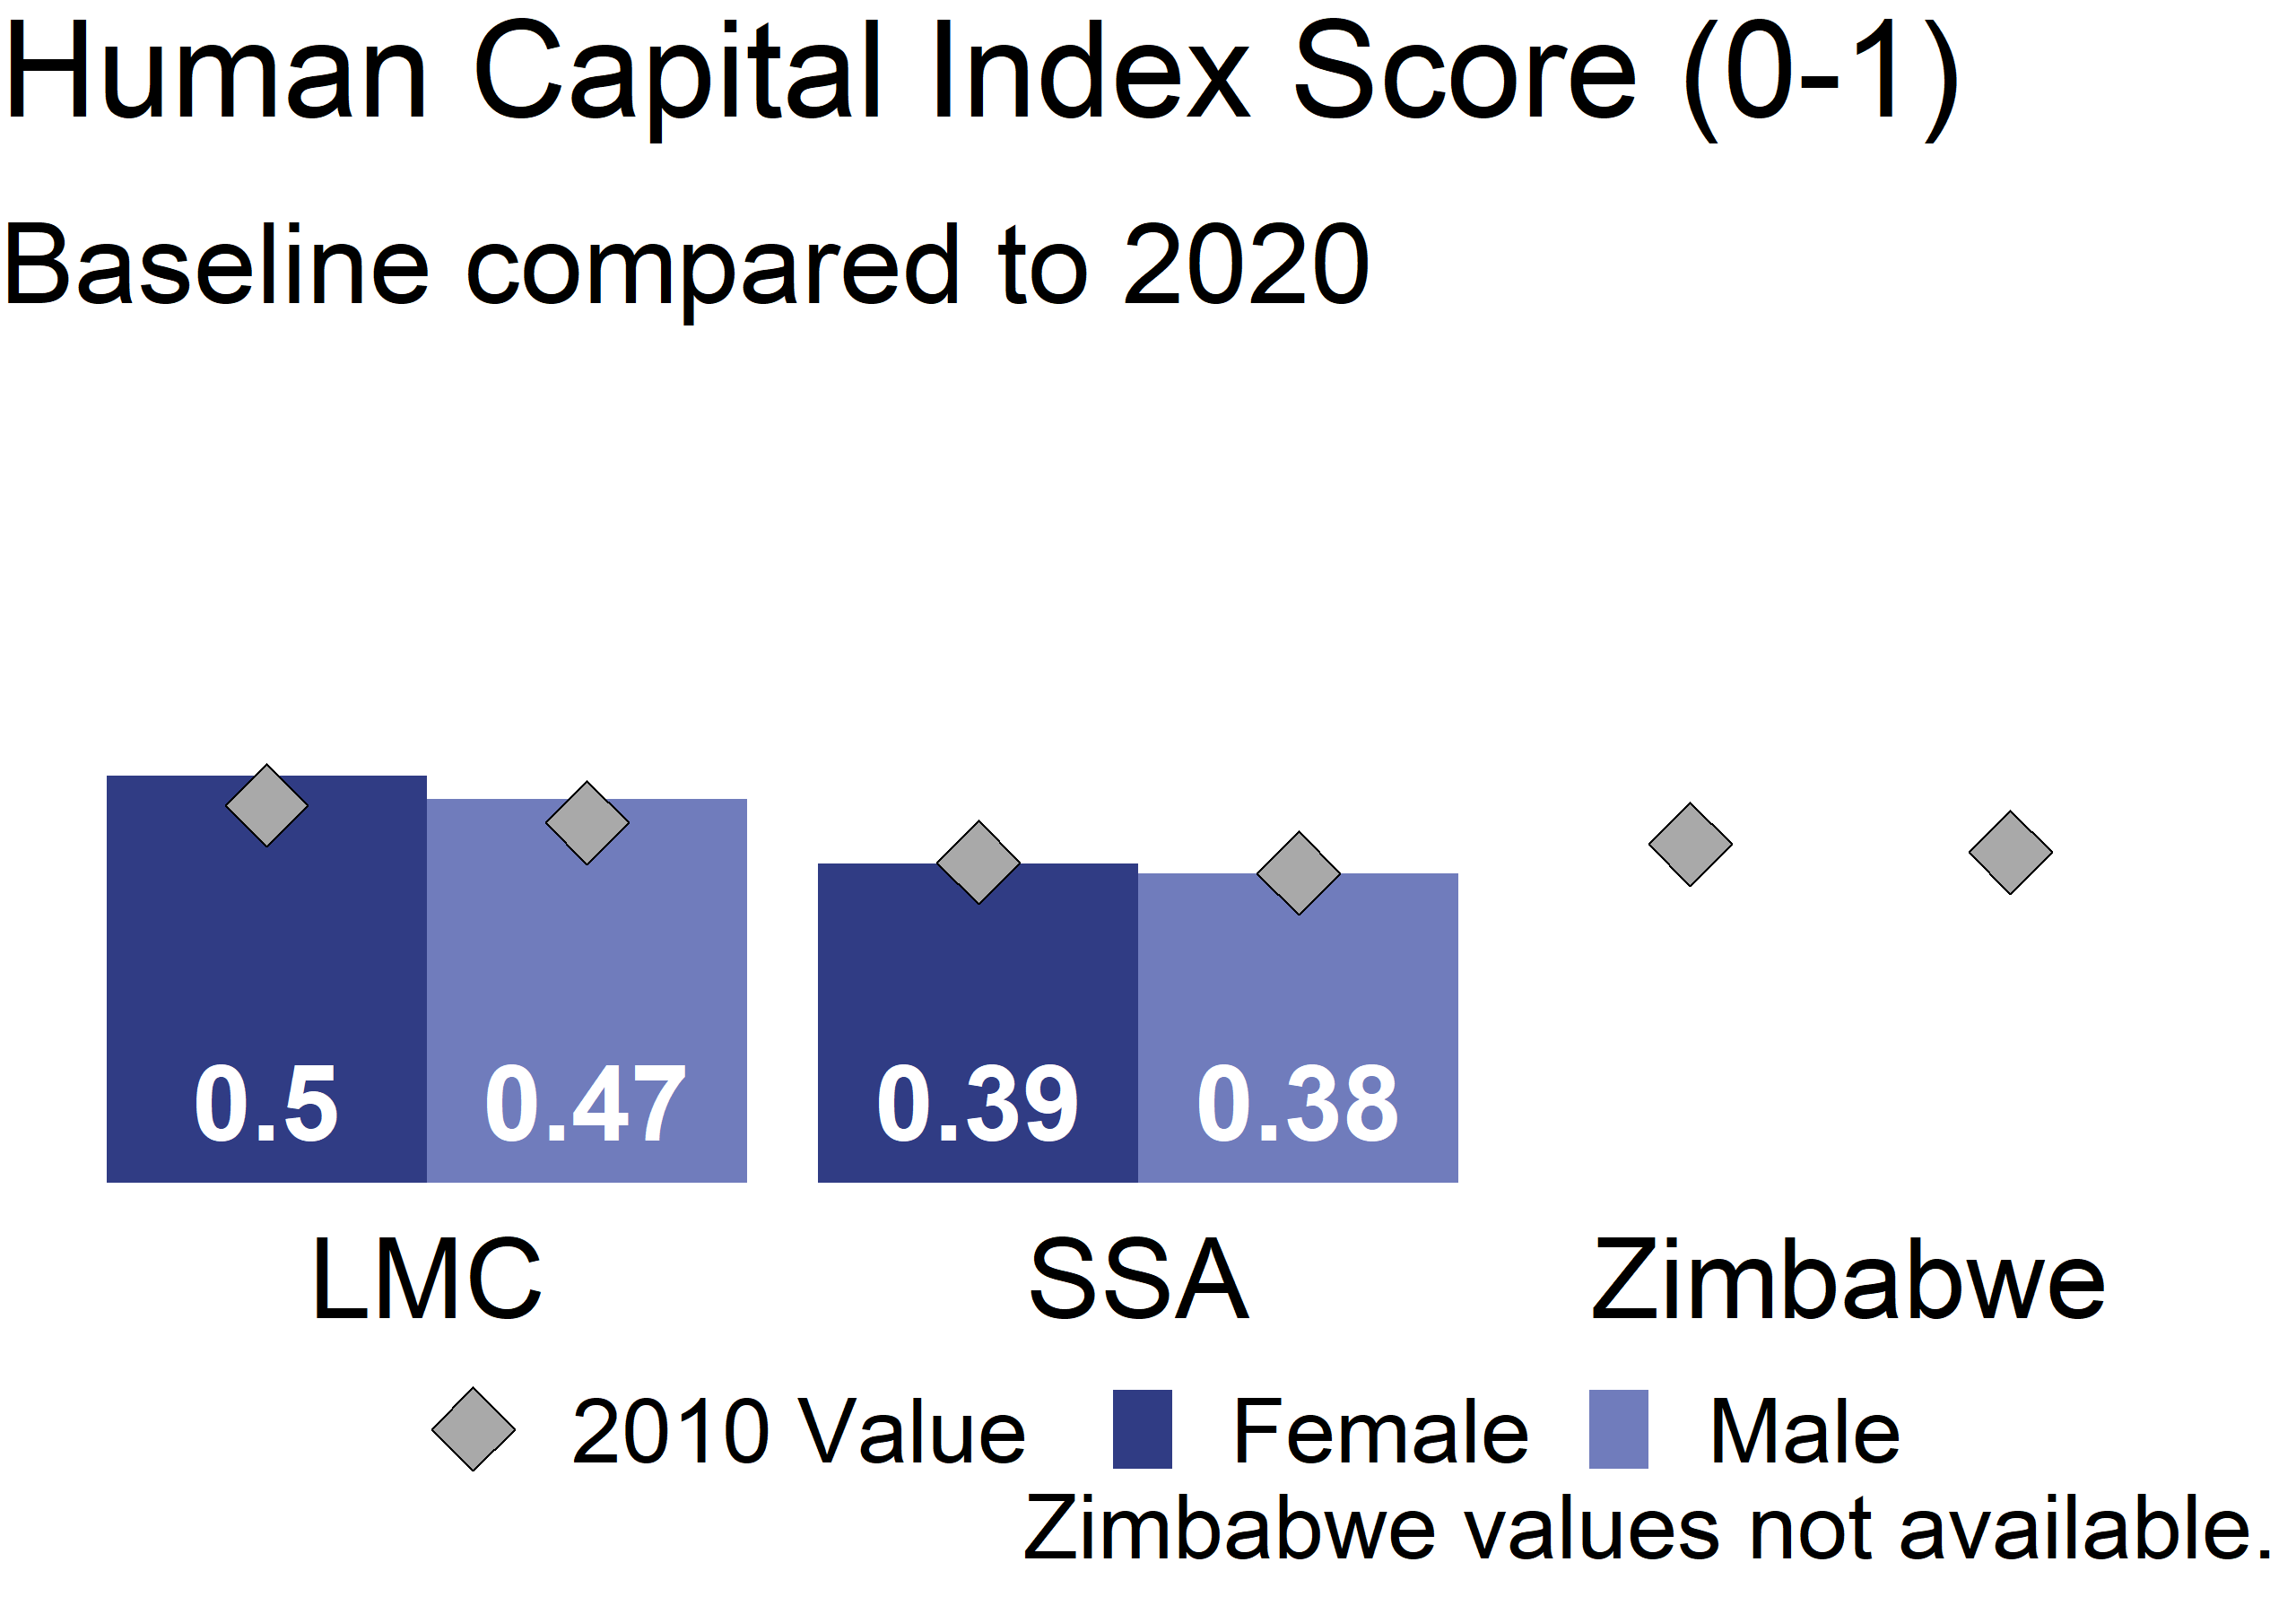
\includegraphics[height=4.7cm]{HCIplot.png}}\hspace{.2cm}
\href{https://genderdata.worldbank.org/indicators/sl-tlf-acti-zs/}{\includegraphics[height=4.7cm]{LFPplot.png}}  
\end{minipage}

\vspace{.2cm}

\centering\fontsize{10}{8}\selectfont

------ \textbf{Unpacking the Numbers in Mozambique} ------ \normalsize

\fboxrule.6pt\fcolorbox{white}{white}{\color{black}
\begin{minipage}[c][3.3cm][t]{3.15cm}
\vspace{.15cm}\fontsize{10}{5}\centering
\href{https://genderdata.worldbank.org/indicators/se-prm-cmpt-zs}{\textbf{55 percent}}

\centering\rule{2.5cm}{0.5pt}
\vspace{.15cm}

\fontsize{9}{5}\selectfont\href{https://genderdata.worldbank.org/indicators/se-prm-cmpt-zs}{A girl has a 45 percent chance of not completing lower secondary school (2020)}
\normalsize\end{minipage}}\hspace{0.45cm}
\fboxrule.6pt\fcolorbox{white}{white}{\color{black}
\begin{minipage}[c][3.3cm][t]{3.15cm}
\vspace{.15cm}\fontsize{10}{5}\centering
\href{https://genderdata.worldbank.org/indicators/sp-2024-fe-zs}{\textbf{1 in 2}}

\centering\rule{2.5cm}{0.5pt}
\vspace{.15cm}

\fontsize{9}{5}\selectfont\href{https://genderdata.worldbank.org/indicators/sp-2024-fe-zs}{46.4 percent of women 15 to 19 years old have had children or already pregnant (2018)}
\normalsize\end{minipage}} \hspace{0.45cm}
\fboxrule.6pt\fcolorbox{white}{white}{\color{black}
\begin{minipage}[c][3.3cm][t]{3.15cm}
\vspace{.15cm}\fontsize{10}{5}\centering
\href{https://genderdata.worldbank.org/indicators/sg-vaw-afsx-zs}{\textbf{6 percent}}

\centering\rule{2.5cm}{0.5pt}
\vspace{.15cm}

\fontsize{9}{5}\selectfont\href{https://genderdata.worldbank.org/indicators/sg-vaw-afsx-zs}{6 percent of women report having ever experienced any form of sexual violence (2015)}
\normalsize\end{minipage}}\hspace{0.45cm}
\fboxrule.6pt\fcolorbox{white}{white}{\color{black}
\begin{minipage}[c][3.3cm][t]{3.15cm}
\vspace{.15cm}\fontsize{10}{5}\centering
\href{https://genderdata.worldbank.org/indicators/sg-dmk}{\textbf{1 in 5}}

\centering\rule{2.5cm}{0.5pt}
\vspace{.15cm}

\fontsize{9}{5}\selectfont\href{https://genderdata.worldbank.org/indicators/sg-dmk}{19.7 percent of women are not able to visit family, relatives and friends on her own decision (2015)}
\normalsize\end{minipage}}\hspace{0.45cm}
\fboxrule.6pt\fcolorbox{white}{white}{\color{black}
\begin{minipage}[c][3.3cm][t]{3.15cm}
\vspace{.15cm}\fontsize{10}{5}\centering

\href{https://genderdata.worldbank.org/indicators/sg-own-ld}{\textbf{41 in 42}}

\centering\rule{2.5cm}{0.5pt}
\vspace{.15cm}

\fontsize{9}{5}\selectfont\href{https://genderdata.worldbank.org/indicators/sg-own-ld}{97.6 percent of women do not have any land, both solely and jointly, registered under their name (2015)}
\normalsize\end{minipage}}

\vspace{.15cm}

\centering\rule{19.5cm}{0.5pt}

\vspace{0.15cm}

\fcolorbox{white}{white}{\color{black}
\raggedright\begin{minipage}[t][5cm][t]{9cm}
\fontsize{10}{12}\selectfont
\textbf{ LEARN MORE}
\fontsize{9}{12}\selectfont

\begin{itemize}
  \item\textbf{\underline{\href{https://www.worldbank.org/en/topic/gender}{The World Bank in Gender}}}: This portal features the latest research, news, and events around gender equality in international development.

  \item\textbf{\underline{\href{https://wbl.worldbank.org/en/wbl}{Women, Business and the Law}}}: This portal includes reports, data, and  news on the laws and regulations that affect women's economic opportunity.
  
  \item\textbf{\underline{\href{https://openknowledge.worldbank.org/handle/10986/23425}{World Bank Group Gender Strategy (FY16-FY23)}}}: This 2015 report outlines the World Bank Group's strategy to promote gender equality.
\end{itemize}

\end{minipage}}
\fcolorbox{white}{white}{\color{black}
\raggedright\begin{minipage}[t][5cm][t]{9cm}
\fontsize{10}{12}\selectfont
\textbf{ }
\fontsize{9}{12}\selectfont

\begin{itemize}
  \item\textbf{\underline{\href{https://genderdata.worldbank.org/}{World Bank Gender Data Portal}}}: This open data page shares the latest statistics and research to improve understanding and inform policy choices.
  
  \item\textbf{\underline{\href{https://www.ifc.org/wps/wcm/connect/Topics_Ext_Content/IFC_External_Corporate_Site/Gender+at+IFC}{IFC Work in Gender}}}: This page provides an overview of the work by IFC to promote gender equality in its global partnerships.
  
  \item\textbf{\underline{\href{https://www.worldbank.org/en/programs/africa-gender-innovation-lab}{AFR Gender Innovation Lab}}}: This page features policy research by the GILs, identifies priority gender gaps and tests innovative solutions in the SSA region.
\end{itemize}

\end{minipage}}

\end{document}
